%\documentstyle[epsf,twocolumn]{jarticle}       %LaTeX2e仕様
\documentclass[twocolumn]{jarticle}     %pLaTeX2e仕様(platex.exeの場合)
%\documentclass[twocolumn]{ujarticle}     %pLaTeX2e仕様(uplatex.exeの場合)
%%%%%%%%%%%%%%%%%%%%%%%%%%%%%%%%%%%%%%%%%%%%%%%%%%%%%%%%%%%%%%
%%
%%  基本バージョン
%%
%%%%%%%%%%%%%%%%%%%%%%%%%%%%%%%%%%%%%%%%%%%%%%%%%%%%%%%%%%%%%%%%
\setlength{\topmargin}{-45pt}
%\setlength{\oddsidemargin}{0cm} 
\setlength{\oddsidemargin}{-7.5mm}
%\setlength{\evensidemargin}{0cm} 
\setlength{\textheight}{24.1cm}
%setlength{\textheight}{25cm} 
\setlength{\textwidth}{17.4cm}
%\setlength{\textwidth}{172mm} 
\setlength{\columnsep}{11mm}

\kanjiskip=.07zw plus.5pt minus.5pt


% 【節が変わるごとに (1.1)(1.2) … (2.1)(2.2) と数式番号をつけるとき】
%\makeatletter
%\renewcommand{\theequation}{%
%\thesection.\arabic{equation}} %\@addtoreset{equation}{section}
%\makeatother

%\renewcommand{\arraystretch}{0.95} 行間の設定

%%%%%%%%%%%%%%%%%%%%%%%%%%%%%%%%%%%%%%%%%%%%%%%%%%%%%%%%
\usepackage[dvipdfmx]{graphicx}   %pLaTeX2e仕様(\documentstyle ->\documentclass)\documentclass[dvipdfmx]{graphicx}
\usepackage[dvipdfmx]{color}
\usepackage[subrefformat=parens]{subcaption}
\usepackage{colortbl}
\usepackage{multicol}
%%%%%%%%%%%%%%%%%%%%%%%%%%%%%%%%%%%%%%%%%%%%%%%%%%%%%%%%

\begin{document}

\twocolumn[
\noindent

\hspace{1em}
2020年10月30日
\hfill
\ \ 細川 岳大

\vspace{2mm}

\hrule

\begin{center}
{\Large \bf 進捗報告}
\end{center}
\hrule
\vspace{3mm}
]

% ‚ここから 文章 Start!

\section{今週やったこと}

\begin{itemize}
	%\item optuna
	\item GAによる疑似ラベルの実験
	\item 予測精度の実験
\end{itemize}

\section{疑似ラベルの実験}
\subsection{設定}
ラベルなし画像100枚取り出し,それらに対するラベルをGAによって探索する.
\ref{tb:GApara}に実験の設定を示す.
目的関数はSVMの精度とした.
ただし,randomforest,4層MLPについても実験をしたが同じような結果のため省く.\\
 遺伝子は0から9の整数値をとる整数値コーディングとした.\\
 選択はサイズ2のトーナメント選択,交叉には二点交叉,突然変異は別の数値にランダムに移るように設定した.\\
 また今回はtrainとevalを固定したものを実験1と,世代ごとに分割しなをしたものを実験2とする.

\begin{table}[h]
	\centering
	\caption{GAの設定\label{tb:GApara}}
	\scalebox{1.0}{
		\begin{tabular}{|c||c|} \hline
			個体数&50\\ \hline
			世代数&70\\ \hline
			交叉率&1.0\\ \hline
			突然変異率&0.02\\ \hline\hline
			全ラベル付き画像&250枚\\ \hline
			train:eval&100枚:150枚\\ \hline
			search&100枚\\ \hline
		\end{tabular}
	}
\end{table}

\subsection{結果}
実験結果を図\ref{fig:ex1},\ref{fig:ex2}に示す.
また散布図を図\ref{fig:ex1:1},\ref{fig:ex1:2},\ref{fig:ex2:1}示す.\\

\begin{figure}[h]
	\begin{center}
		\centering
		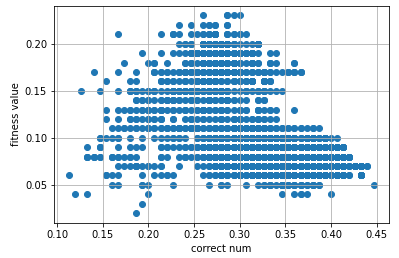
\includegraphics[scale=0.5]{ex4_all.png}
		\caption{実験1の散布図\label{fig:ex1:1}}
	\end{center}
\end{figure}
\begin{figure}[h]
	\begin{center}
		\centering
		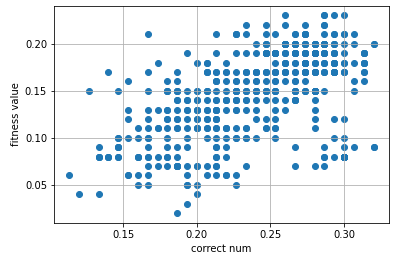
\includegraphics[scale=0.5]{ex4_first10.png}
		\caption{実験1の散布図(10世代まで)\label{fig:ex1:2}}
	\end{center}
\end{figure}
\begin{figure}[bh]
	\begin{center}
		\centering
		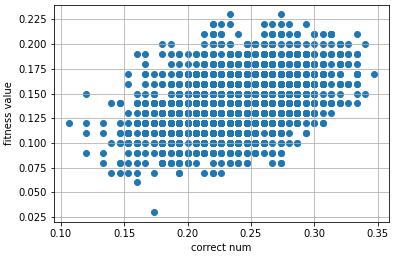
\includegraphics[scale=0.5]{ex8_all.png}
		\caption{実験2の散布図\label{fig:ex2:1}}
	\end{center}
\end{figure}
\clearpage

図から実験1はfitnessがは上がり続けているが実際の正答率は下がっており過学習が見て取れるのに対し,実験2では世代ごとのfitnessはぶれてはいるものの実際の正答率は上がっているのが分かる.\\
また散布図からも実験1で10世代まで取り出したものでは相関性があるように思われる.
実験2の散布図においても若干の相関性がありそうであり,evalの画像が変わっているために幅が広くなっているのではないかと思われる.

\section{ランダムなラベルの割合と精度}
\subsection{設定}
前回の結果からランダムなラベルの割合に対する頑健性を調べた.
表\ref{tb:FTXpara}に設定を示す.
今回は1\%2\%10\%20\%30\%の割合の時について調べた.
また時間の都合上2回ずつしか回していない.
\begin{table}[h]
	\centering
	\caption{FixMatchの設定\label{tb:FTXpara}}
	\scalebox{1.0}{
		\begin{tabular}{|c|c|c|} \hline
			model&\multicolumn{2}{c|}{WideResNet28-2}\\ \hline\hline
			data set&\multicolumn{2}{c|}{cifar10}\\ \hline
			train &labeled+random&500\\ \cline{2-3}
			data&unlabeled&49650\\ \hline
			batch size&labeled+random&64\\ \cline{2-3}
			&unlabeled&$64*7$\\ \hline
			val data&\multicolumn{2}{c|}{10000}\\ \hline\hline
			num\_iterations&\multicolumn{2}{c|}{2**14}\\ \hline
			optimizer&\multicolumn{2}{c|}{SGD(lr=0.1,momntum=0.9)}\\ \hline
			loss&\multicolumn{2}{c|}{cross\_entropy\_loss}\\ \hline
		\end{tabular}
	}
\end{table}

\subsection{結果}
表\ref{tb:res2}に結果を示す.
\begin{table}[h]
	\centering
	\caption{GAの設定\label{tb:res2}}
	\scalebox{1.0}{
		\begin{tabular}{|c||c|c|c|c|c|} \hline
			&1\%&2\%&10\%&20\%&30\%\\ \hline\hline
			1回目&0.1799&0.3693&0.1631&0.1338&0.1362\\ \hline
			2回目&0.2034&0.1603&0.1681&0.1755&0.1545\\ \hline
		\end{tabular}
	}
\end{table}

試行回数が少ないが,精度についてランダムなラベルの割合というよりも
データの種類による影響の方が大きいように感じる.またいずれにせよ精度についてほぼ20\%
以下であり,GAの実験としてもう少し違う設定にしなければならないようにも思われる.

\section{予測精度の実験}
前回言っていた,予測された確率とラベルに対する精度について調べた.
表\ref{tb:FMpara}に設定を示す.\\
\begin{table}[h]
	\centering
	\caption{FixMatchの設定\label{tb:FMpara}}
	\scalebox{1.0}{
		\begin{tabular}{|c|c|} \hline
			model&WideResNet16-2\\ \hline\hline
			data set&cifar10\\ \hline
			labeled data&250\\ \hline
			unlabeled data&49750\\ \hline
			batch(labeled)&64\\ \hline
			batch(unlabeled)&$64*7$\\ \hline
			val data&10000\\ \hline\hline
			num\_iterations&40000\\ \hline
			optimizer&SGD(lr=0.1,momntum=0.9)\\ \hline
			loss&cross\_entropy\_loss\\ \hline
		\end{tabular}
	}
\end{table}
結果については同階層の画像を参照.

\section{考えていること}
GAを用いてラベルを予測するのは厳しいと思われるので,ある程度学習して予測したものに対し,閾値を設けてそれらを疑似ラベルとして採用したうえで,それらを使うか否かをGAによって探索する.
意味があるかどうかはわからないが,モデルの入力に画像とラベルを入れ,出力をその組み合わせが正しいかどうかとし,もともとのラベル付きに対する出力が0か1,ラベルなしに対しては全ての出力を0.1のようにし,異常検出の容量でラベルをつけることはできないかどうか.

\begin{figure}[tp]
	\begin{center}
		\centering
		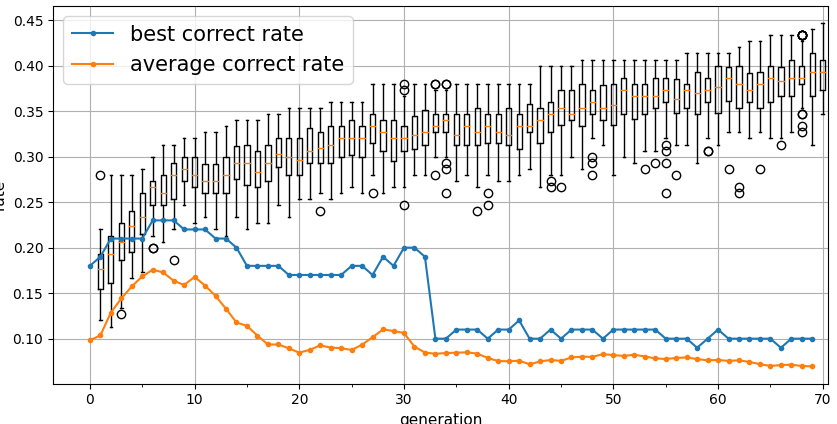
\includegraphics[scale=0.7]{ex4_graph2.png}
		\caption{実験1結果\label{fig:ex1}}
	\end{center}
\end{figure}

\begin{figure}[tp]
	\begin{center}
		\centering
		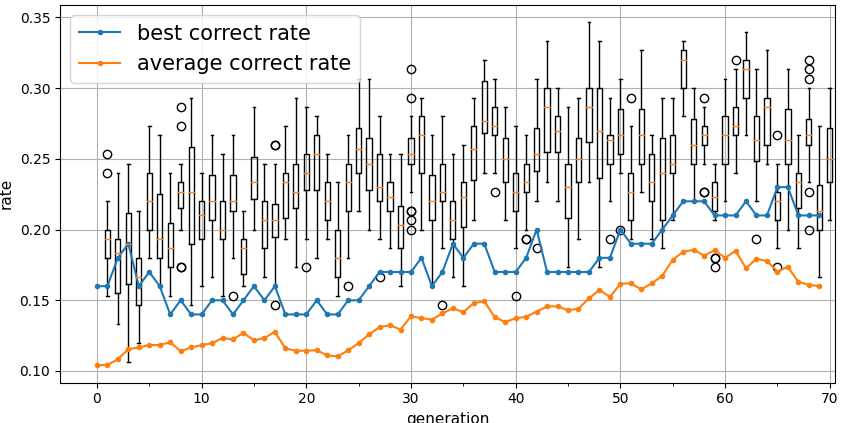
\includegraphics[scale=0.7]{ex8_graph2.png}
		\caption{実験2結果\label{fig:ex2}}
	\end{center}
\end{figure}


\end{document}


